\chapter{MLops}
Una tipica pipeline per un progetto di machine learning è composta da diverse fasi:
\begin{itemize}
    \item Comprensione del problema
    \item Raccolta dei dati
    \item Comprensione dei dati
    \item Preparazione dei dati
    \item Modellazione
    \item Valutazione
    \item Deployment
\end{itemize}
\begin{figure}[!ht]
    \centering
    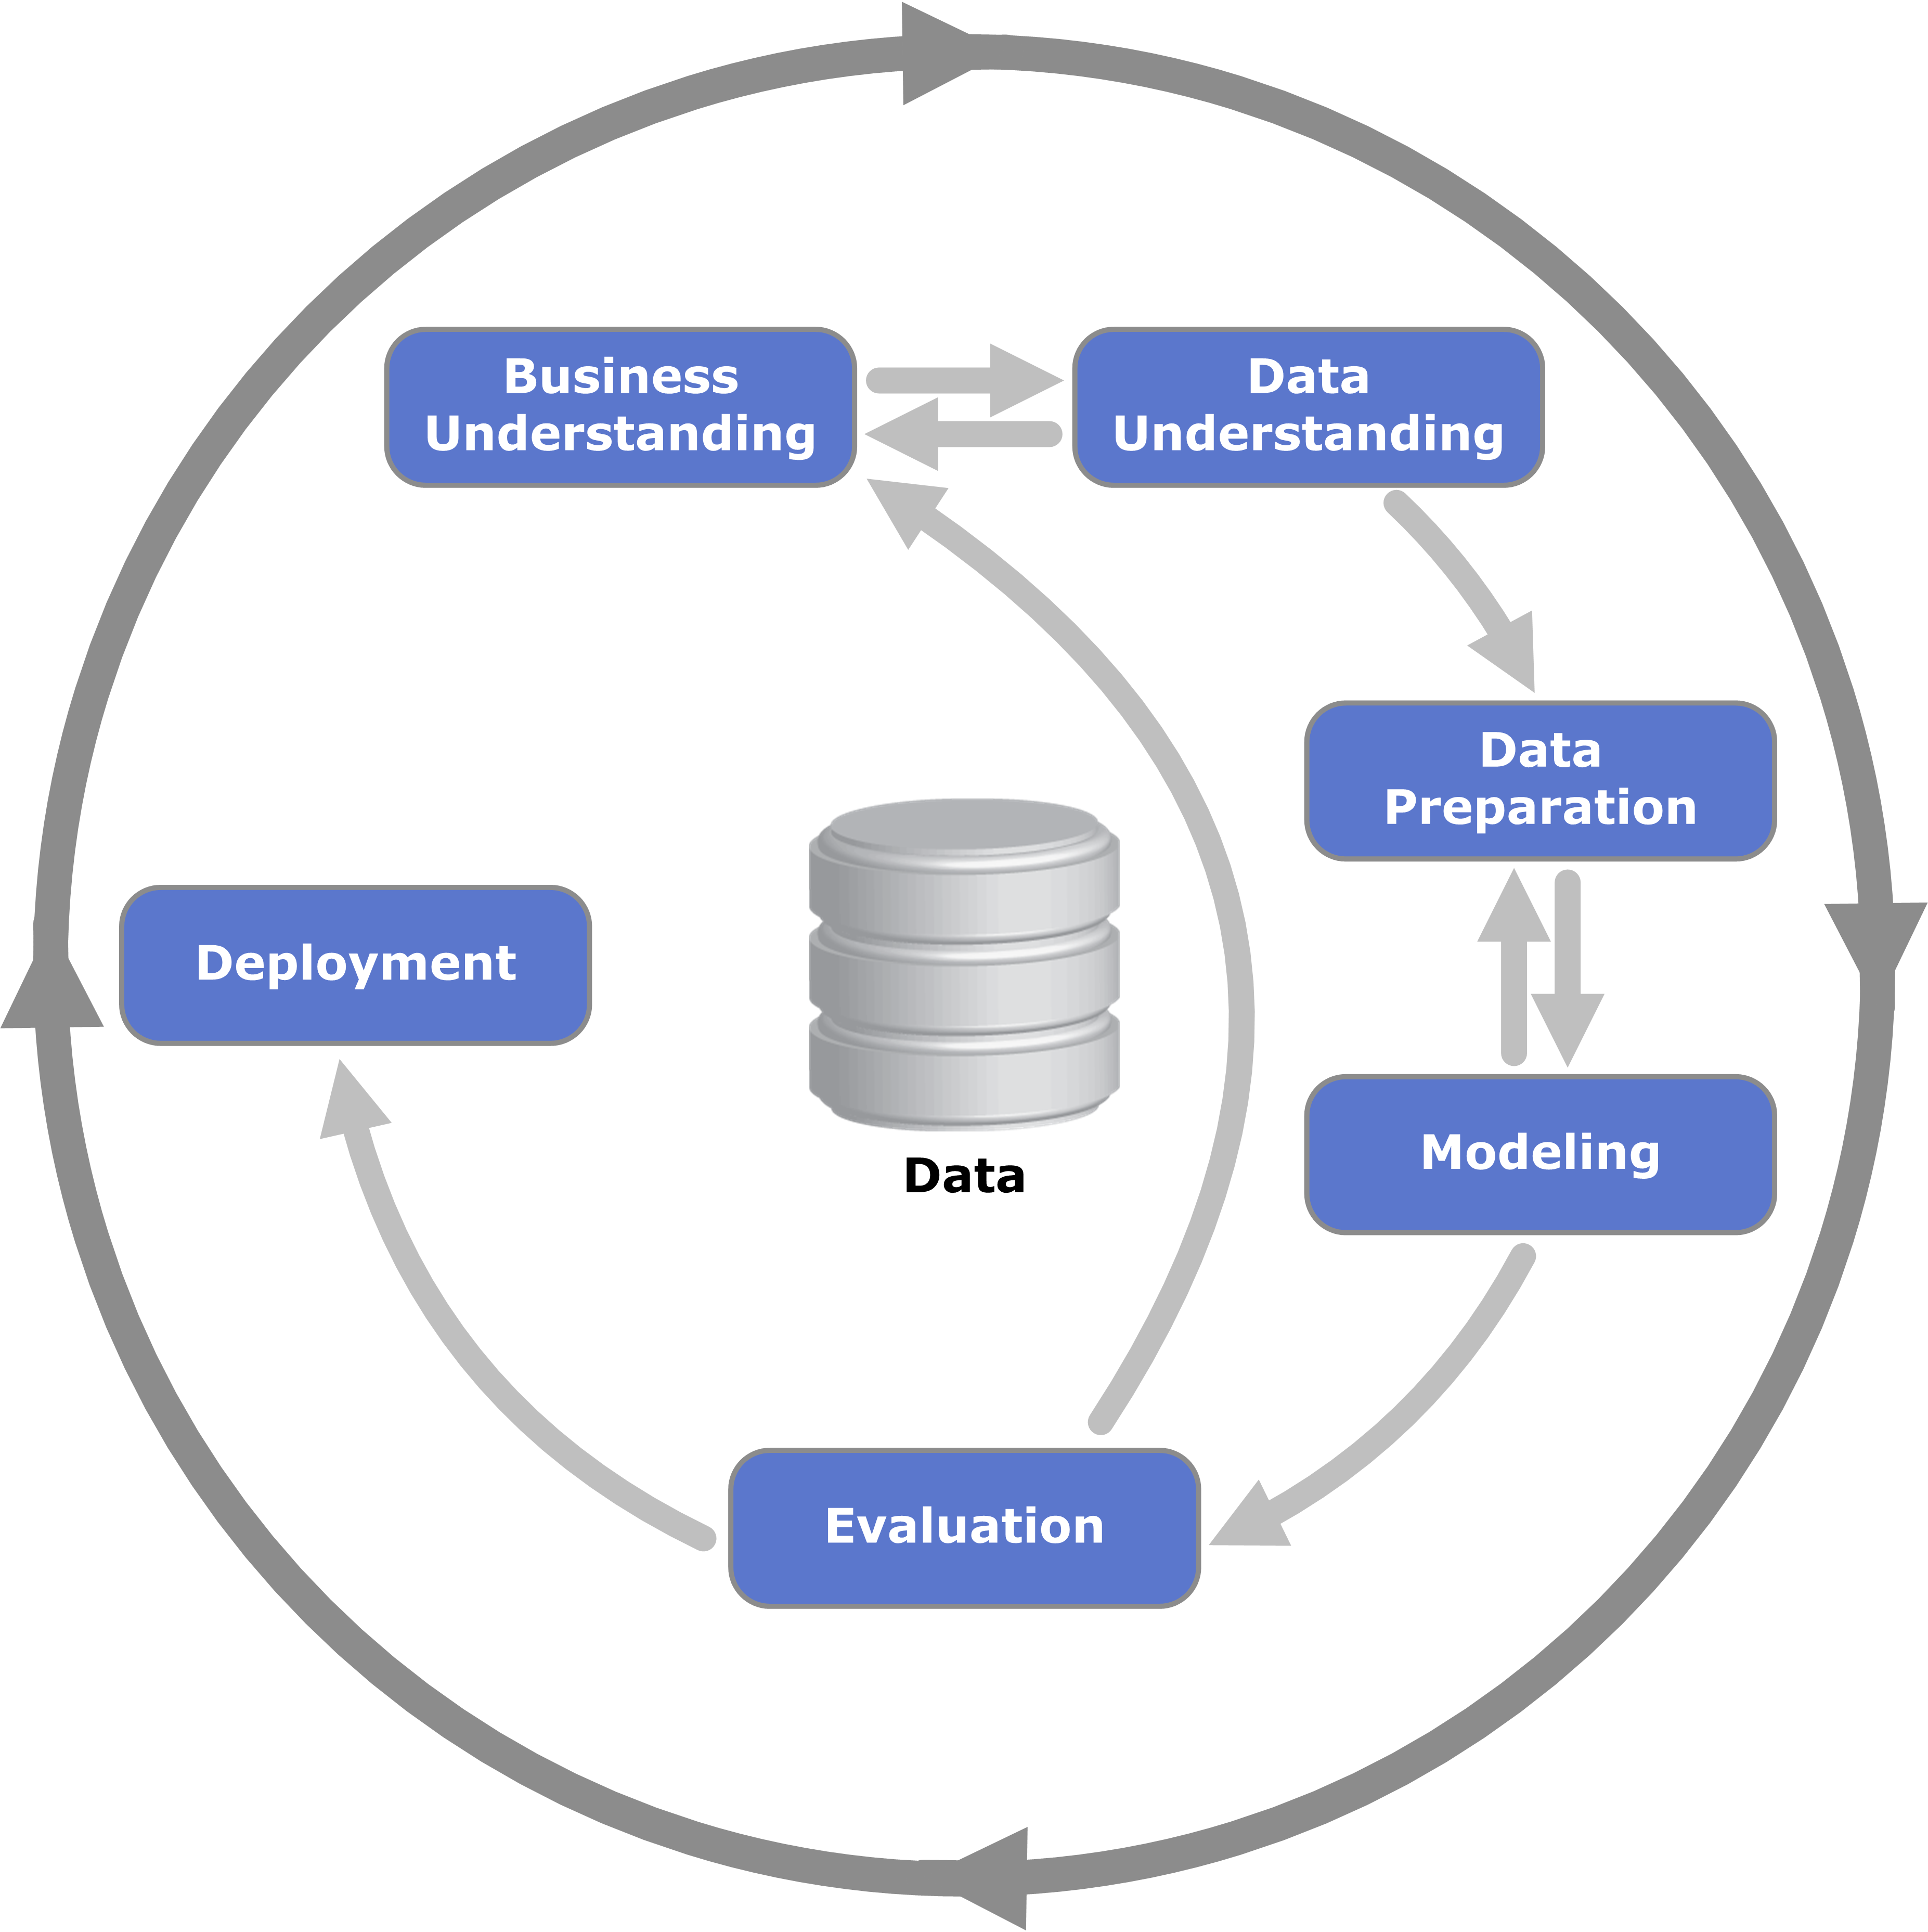
\includegraphics[width=0.5\textwidth]{./img/MLops/CRISP-DM.png}
    \caption{ML Pipeline}
    \label{fig:ml_pipeline}
\end{figure}
In questa parte del corso ci occuperemo della parte di gestione dei dati, nello
specifico analizzeremo la parte di \textbf{Data Understanding} e \textbf{Data
    Preparation}.

Avere i dati corretti è una parte fondamentale per la creazione di un modello di
che sia in grado di ottenere dei risultati corretti.
\begin{center}
    \textit{Garbage in, garbage out}
\end{center}
I dati di training e testing devono derivare dai dati reali che verranno raccolti
in fase di production.
\section{Pipeline}
Una volta ottenuti i dati reali dovremo separarli in:
\begin{itemize}
    \item \textbf{Training data}: vengono utilizzati per addestrare e valutare
          il modello, sono quindi di dimensioni elevate e vengono raccolti
          attraverso diverse fonti. Spesso caratterizzati da un elevato throughput.
    \item \textbf{Serving data}: raccolti e utilizzati per fare previsioni in
          fase di production. Questa tipologia di dati è spesso caratterizzata
          da una bassa latenza.
\end{itemize}
Entrambi questi tipi di dati devono passare attraverso una fase di preparazione.
In questa fase si vogliono stabilire quali sono le informazioni principali,
quali dati sono rilevanti e quali dati sono irrilevanti. Si effettua dunque una
prima analisi. Inoltre, vengono eseguite diverse operazioni per far si che i dati
si adattino al modello che si vuole creare.

Prima di arrivare alla parte di addestramento del modello, si passa attraverso una
fase di validazione dei dati. Quest fase è necessaria in quanto i dati cambiano
o cambia il contesto.

L'obiettivo principale è quello di capire quali feature sono significative
per il modello e quali no. Questo serve per controllare in futuro se queste
feature significative sono cambiate.

Questa fase viene fatta confrontando le distribuzioni delle features ritenute
significative durante il training con la distribuzione delle stesse feature prese
dai dati raccolti in produzione.

In questo modo possiamo segnalare quando le distribuzioni cambiano e nel caso devo
adottare delle soluzioni:
\begin{itemize}
    \item Riaddestrare il modello.
    \item Avvisare l'utente che qualcosa sta cambiando.
    \item Non fare niente.
\end{itemize}
Può capitare nel tempo i le feature cambino il tipo (ad esempio si passa da int
a float), quindi, nella fase di validation, bisogna correggerli per renderli
compatibili col modello.

Per effettuare tutti i passi della pipeline servono diverse figure lavorative:
\begin{itemize}
    \item \textbf{Machine Learning Expert}
    \item \textbf{Software Engineer}
    \item \textbf{Site Reliability Engineer}: esperto che si occupa di gestire
          tutta la pipeline e di risolvere eventuali problemi.
\end{itemize}
\section{Data Acquisition}
Una delle fasi più importanti è \textbf{Data Acquisition}. In questa fase possiamo
avere diversi problemi come ad esempio l'introduzione di bias nei dati che
invalidano i risultati del modello.

In aggiunta, è obbligatorio sapere la \textbf{Data Provenance} ovvero documentare
come ho costruito il dataset di training e validation. Questo consiste nel sapere
quali sono i dati utilizzati, da dove vengono, come ho costruito il dataset. In
questo modo si risolvono eventuali problemi dovuti a risultati sballati per dati
che sono stati iniettati nel dataset.